\documentclass[compress,mathserif]{beamer}

\usepackage{amssymb}
\usepackage{amsfonts}
\usepackage{amsmath}
\usepackage{amsxtra}
\usepackage{hyperref}
\usepackage{tensor}
\usepackage{dsfont}

\mode<presentation> {
  \usetheme{default}
  \useoutertheme{infolines}
  \setbeamercovered{transparent}
  \beamertemplateballitem
}

\title[Claim Severity Models]{Severity Models - Special Families of Distributions}
\author{Sections 5.3-5.4}
\institute[Stat 346]{Stat 346 - Short-term Actuarial Math}
\date[BYU]{}
\subject{Stat 477}

\begin{document}

\begin{frame}
 \titlepage
\end{frame}

\section{Introduction}
\frame{\frametitle{Introduction}
\begin{itemize}
\item Given that a claim occurs, the (individual) claim size $X$ is typically referred to as \alert{claim severity}.
\smallskip
\item While typically this may be of continuous random variables, sometimes claim sizes can be considered discrete.
\smallskip
\item When modeling claims severity, insurers are usually concerned with the tails of the distribution. There are certain types of insurance contracts with what are called \alert{long tails}.
\end{itemize}
}

\subsection{parametric class}
\frame{\frametitle{Parametric distributions}
A \alert{parametric distribution} consists of a set of distribution functions with each member determined by specifying one or more values called ``parameters''. \\
\smallskip
The parameter is fixed and finite, and it could be a one value or several in which case we call it a vector of parameters. Parameter vector could be denoted by $\theta$. \\
}

\frame{\frametitle{Parametric distributions}
Some parameters have special names:
\begin{itemize}
\item Location parameters: controls the shift of the distribution. If $f(x-\mu)$ belongs to the same family of distribution as $f$ then $f$ is called a location family and $\mu$ is a location parameter.
\item Scale parameter: controls the spread of the distribution. If $\frac{1}{\sigma}f\left(\frac{x}{\sigma}\right)$ belongs to the same family as $f$, then $f$ is a scale distribution and $\sigma$ is a scale parameter. 
\item Note: a distribution where $\frac{1}{\sigma}f\left(\frac{x-\mu}{\sigma}\right)$ belongs to the same family as $f$ is called a location scale family. 
\item Rate parameter: For some distributions you can have a rate parameter which is the inverse of the scale parameter $1/\sigma$
\item Shape parameter: All parameters that are not location or scale parameters and are not functions of location and scale parameter is called a shape parameter. 
\end{itemize}
%The \alert{Normal} distribution is a clear example:
%\begin{equation*}
%f_X(x) = \frac{1}{\sqrt{2\pi}\sigma} e^{-(x-\mu)^2/2\sigma^2},
%\end{equation*}
%where the parameter vector $\theta = (\mu,\sigma)$. It is well known that $\mu$ is the mean and $\sigma^2$ is the variance. Some important properties:
%\begin{itemize}
%\item Standard Normal when $\mu=0$ and $\sigma=1$.
%\item If $X \sim \text{N}(\mu,\sigma)$, then $Z = \frac{X-\mu}{\sigma} \sim \text{N}(0,1)$.
%\item Sums of Normal random variables is again Normal.
%\item If $X \sim \text{N}(\mu,\sigma)$, then $cX \sim \text{N}(c\mu,c\sigma)$.
%\end{itemize}
}

\subsection{some claim size distributions}
\frame{\frametitle{Some parametric claim size distributions}
\begin{itemize}
\item Normal - easy to work with, but careful with getting negative claims. Insurance claims usually are never negative.
\smallskip
\item Gamma/Exponential - use this if the tail of distribution is considered `light'; applicable for example with damage to automobiles.
\smallskip
\item Lognormal - somewhat heavier tails, applicable for example with fire insurance.
\smallskip
\item Burr/Pareto - used for heavy-tailed business, such as liability insurance.
\smallskip
\item Inverse Gaussian - not very popular because complicated mathematically.
\end{itemize}
}

\frame{\frametitle{Most distributions are connected}
\begin{center}
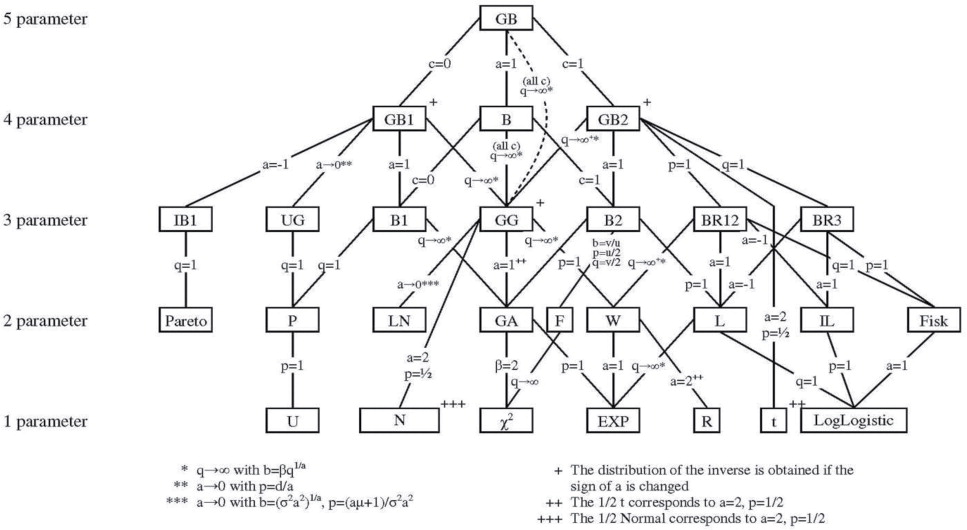
\includegraphics[width=12.5cm,height=6.5cm]{gb.jpg}
\end{center}
}

\subsection{Normal}
\frame{\frametitle{The Normal distribution}
The \alert{Normal} distribution is a clear example:
\begin{equation*}
f_X(x) = \frac{1}{\sqrt{2\pi}\sigma} e^{-(x-\mu)^2/2\sigma^2},
\end{equation*}
where the parameter vector $\theta = (\mu,\sigma)$. It is well known that $\mu$ is the mean and $\sigma^2$ is the variance. 

\smallskip
Some important properties:
\begin{itemize}
\item Standard Normal when $\mu=0$ and $\sigma=1$.
\item If $X \sim \text{N}(\mu,\sigma)$, then $Z = \frac{X-\mu}{\sigma} \sim \text{N}(0,1)$.
\item Sums of Normal random variables is again Normal.
\item If $X \sim \text{N}(\mu,\sigma)$, then $cX \sim \text{N}(c\mu,c\sigma)$.
\end{itemize}
}

\section{Some familiar distributions}
\subsection{Lognormal}
\frame{\frametitle{The Lognormal distribution}
\begin{itemize}
\item If $Y \sim \text{Normal}(\mu,\sigma)$, then $X = \exp(Y)$ is \alert{lognormal} and we write $X\sim$ Lognormal$(\mu,\sigma)$. Its density can be expressed as
\begin{equation*}
f_X(x) =\frac{1}{x \sigma \sqrt{2\pi}}e^{-(\log x -\mu)^2/2\sigma^2}, \ \ \text{for } x>0.
\end{equation*}
\item Thus, if $X$ is lognormal, then $\log(X)$ is Normal.
\smallskip
\item Moments: $\text{E}(X^k) = \exp(k\mu + k^2 \sigma^2/2)$
\smallskip
\item Mean: $\text{E}(X) =e^{\mu + \sigma^2/2}$ \ \ \ \ Variance:
$\text{Var}(X)=(e^{\sigma^2}-1)e^{2\mu+\sigma^2}$
\smallskip
\item Derive the mode.
\end{itemize}
}

\frame{\frametitle{Lognormal densities for various $\sigma$'s}
\begin{center}
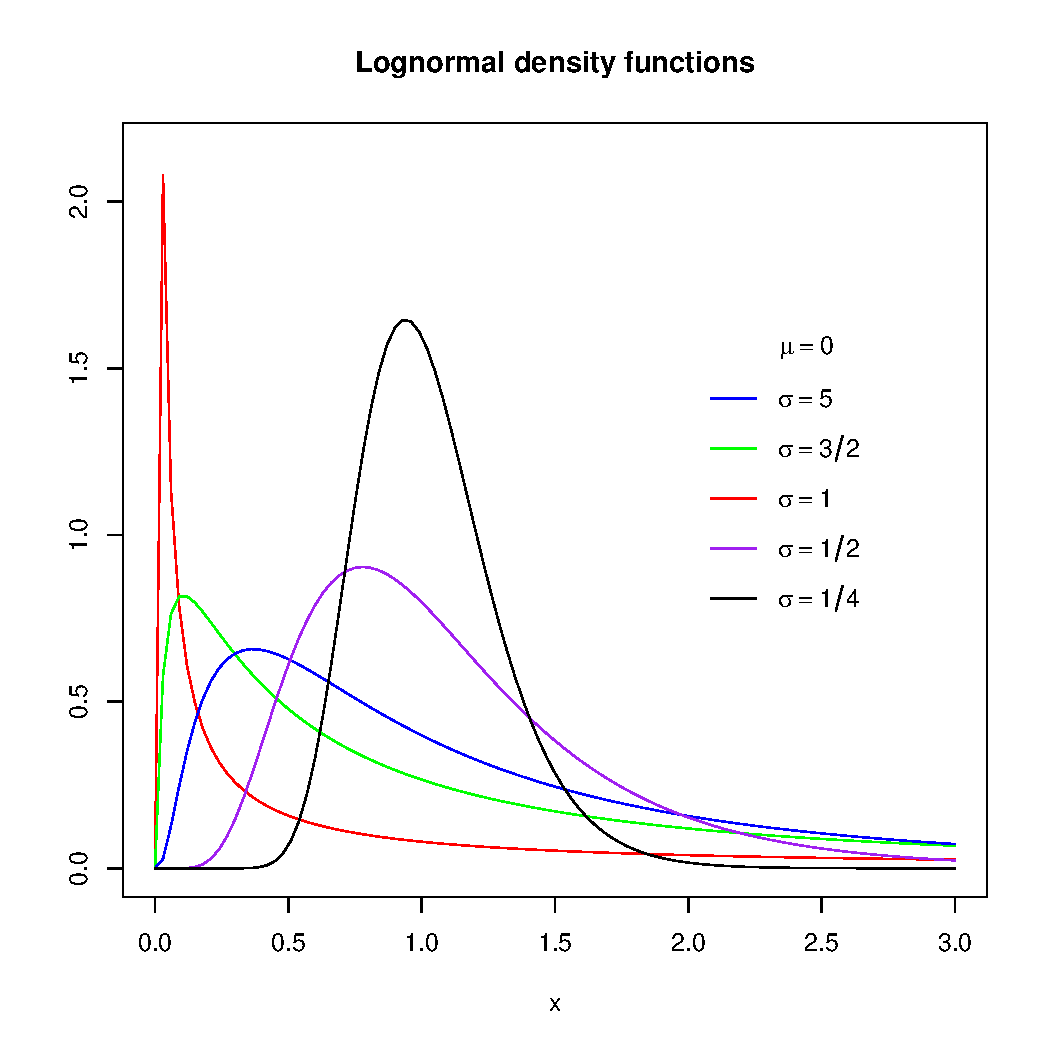
\includegraphics[width=8.5cm,height=6.5cm]{Lect3-Fig1.pdf}
\end{center}
}



\subsection{Gamma}
\frame{\frametitle{The Gamma distribution}
\begin{itemize}
\item We shall write $X\sim $ \alert{Gamma}$(\alpha,\theta)$ if density has the form
\begin{equation*}
f_X(x) =\frac{1}{\theta^\alpha \Gamma(\alpha)} x^{\alpha-1}e^{-x/\theta}, \ \ \text{for } x>0 \text{; }\alpha ,\theta>0,
\end{equation*}
with $\alpha$, the shape parameter, and $\theta$, the scale parameter.
\smallskip
\item Higher moments: $\text{E}(X^{k}) = \dfrac{\Gamma(\alpha+k)}{\Gamma(\alpha)} \theta^k$
\smallskip
\item Mean: $\text{E}(X) =\alpha \theta$ \ \ \ \ Variance: $\text{Var}(X)=\alpha \theta^2$
\smallskip
%\item Moment generating function: $M_X(t)=(1-\theta t)^{-\alpha}$, provided $t<1/\theta$.
\item Special cases:
\begin{itemize}
\item \alert{Exponential}: When $\alpha =1$, we have $X \sim$ Exp $(\theta)$.
\item \alert{Chi-square}: When $\alpha=n/2$ and $\theta=2$, we have a chi-squared distribution with $n$ degrees of freedom.
\end{itemize}
\end{itemize}
}




\subsection{Pareto}
\frame{\frametitle{The Pareto distribution}
\begin{itemize}
\item We shall write $X\sim$ \alert{Pareto}$(\alpha,\theta)$ if density has the form
\begin{equation*}
f_X(x) = \frac{\alpha \theta^{\alpha}}{(x+\theta)^{\alpha+1}}, \ \ \text{for } x>0,
\end{equation*}
where $\alpha>0$ and $\theta>0$.
\smallskip
\item $\alpha$, the shape parameter;  $\theta$, the scale parameter.
\smallskip
\item CDF: $F_X(x) = 1 - \biggl(\dfrac{\theta}{x+\theta}\biggr)^\alpha$.
\smallskip
\item Mean: $\text{E}(X)= \dfrac{\theta}{\alpha-1}$
\smallskip
\item Higher moments: $\text{E}(X^k) = \dfrac{\Gamma(\alpha-k)}{\Gamma(\alpha)} \theta^k \Gamma(k+1), \ \ \text{for } -1<k<\alpha$.
\smallskip
\item Variance: (derive it!)
\smallskip
\end{itemize}
}

\frame{\frametitle{Pareto densities for various $\alpha$'s}
\begin{center}
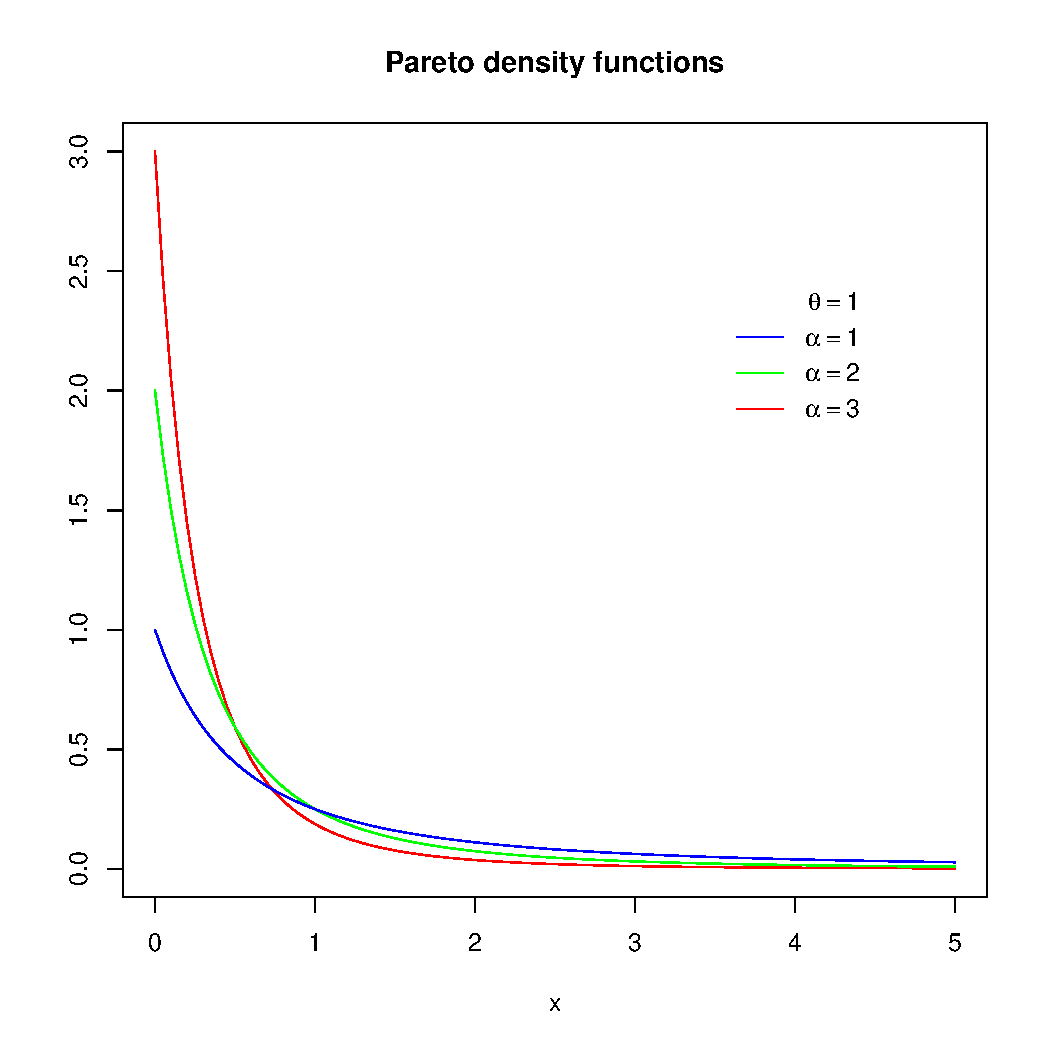
\includegraphics[width=8.5cm,height=6.5cm]{Lect3-Fig2.pdf}
\end{center}
}

\frame{\frametitle{Some important properties}
\begin{itemize}
\item A positive scalar multiple of a Pareto is again a Pareto.
\smallskip
\begin{itemize}
\item If $X \sim \text{Pareto}(\alpha,\theta)$ and $c$ is a positive constant, then $cX \sim \text{Pareto}(\alpha,c \theta)$.
\smallskip
\item This also explains why $\theta$ is called the scale parameter.
\end{itemize}
\smallskip
\item The Pareto distribution is a continuous mixture of exponentials with Gamma mixing weights.
\smallskip
\begin{itemize}
\item If $(X|\Lambda=\lambda) \sim \text{Exp}(1/\lambda)$ and $\Lambda \sim \text{Gamma}(\alpha,1/\theta)$, then unconditionally, $X \sim \text{Pareto}(\alpha,\theta)$.
\smallskip
\item To be derived in lecture - also part of generating new distributions.
\end{itemize}
\end{itemize}
}

\subsection{Burr}
\frame{\frametitle{The Burr distribution}
\begin{itemize}
\item We shall write $X\sim$ \alert{Burr}$(\alpha,\theta,\gamma)$ if density has the form
\begin{equation*}
f_X(x) = \frac{\alpha \gamma (x/\theta)^{\gamma}}{x[1+(x/\theta)^\gamma]^{\alpha+1}}, \ \ \text{for } x>0,
\end{equation*}
where $\alpha>0$, $\theta>0$ and $\gamma>0$.
\smallskip
\item $\alpha$, the shape parameter;  $\theta$, the scale parameter.
\smallskip
\item Sometimes more precisely called \alert{Burr Type XII} distribution and the Pareto is a special case when $\gamma=1$.
\smallskip
\item Higher moments: $\text{E}(X^k)= \dfrac{\Gamma(1+k/\gamma) \Gamma(\alpha-k/\gamma)}{\Gamma(\alpha)} \theta^k$, provided $-\gamma<k<\alpha \gamma$.
\end{itemize}
}

\frame{\frametitle{Burr densities for various parameter values}
\begin{center}
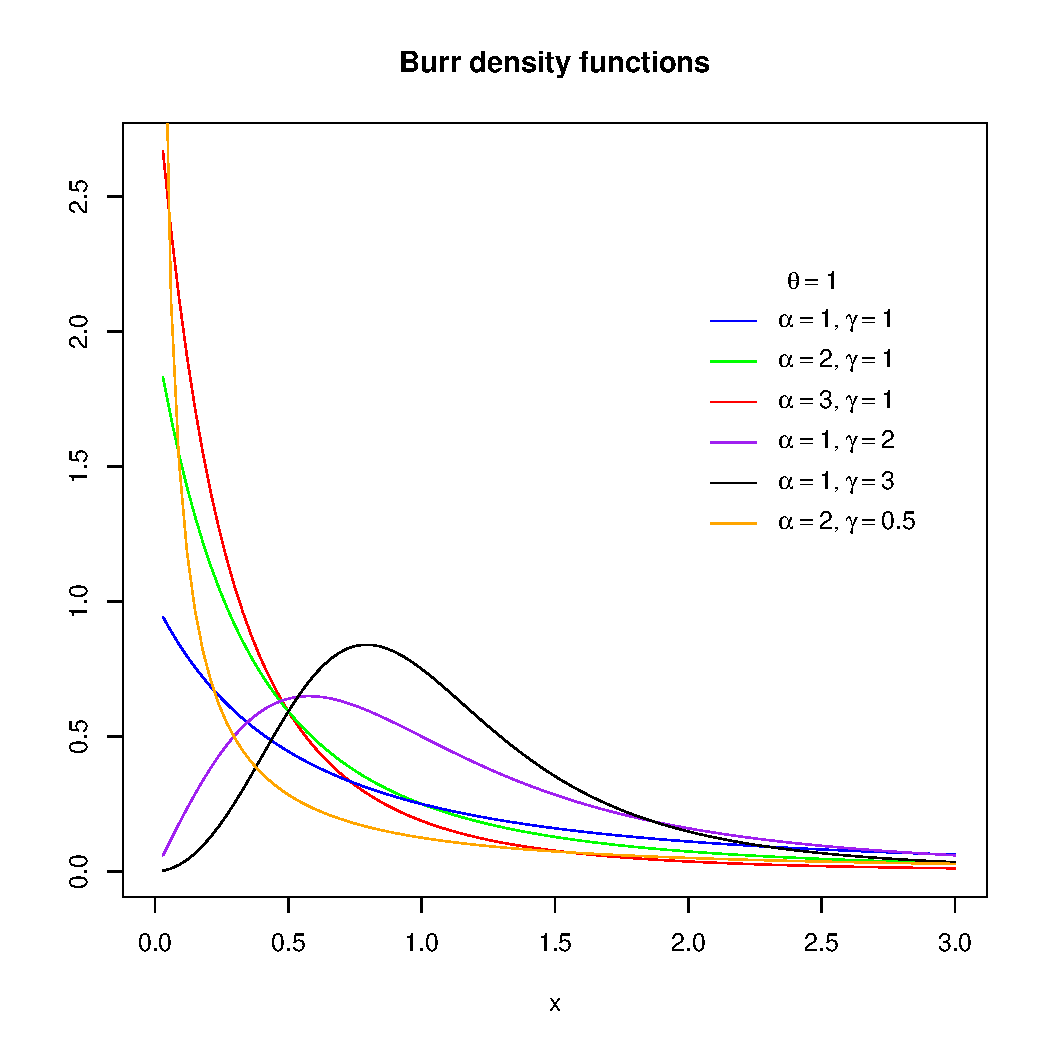
\includegraphics[width=8.5cm,height=6.5cm]{Lect3-Fig3.pdf}
\end{center}
}

\section{Weibull Distribution}
\frame{\frametitle{Weibull Distribution}
\begin{itemize}
\item The Weibull distribution is commonly used in reliability analysis and extreme value modeling.
\smallskip
\item It is characterized by two parameters: 
  \begin{itemize}
  \item Shape parameter ($\tau$) controls the shape of the distribution.
  \item Scale parameter ($\theta$) controls the scale or rate at which events occur.
  \end{itemize}
\smallskip
\item The probability density function (PDF) of the Weibull distribution is given by:
\begin{equation*}
f_X(x) = \frac{\tau \left(\frac{x}{\theta}\right)^{\tau} e^{-(x/\theta)^\tau}}{x}, \quad x \geq 0
\end{equation*}
\end{itemize}
}

\frame{\frametitle{Weibull densities for various parameter values}
\begin{center}
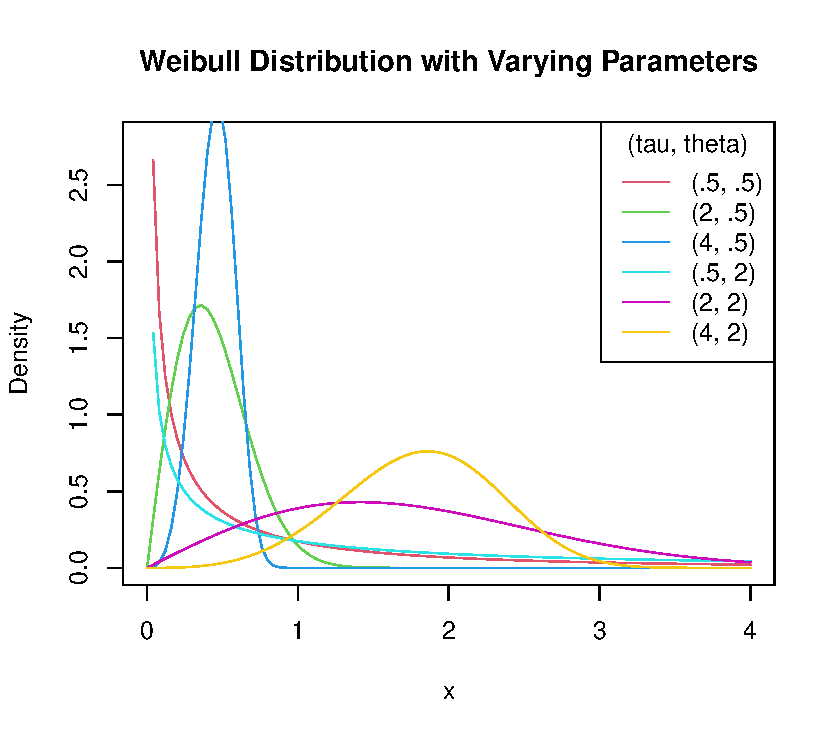
\includegraphics[width=8.5cm,height=6.5cm]{weibull.pdf}
\end{center}
}

\section{Inverse Distributions}
\frame{\frametitle{Inverse Distributions}
\begin{itemize}
\item Inverse distributions are a class of probability distributions that are less common but offer valuable modeling options in severity models.
\smallskip
\item They are known for being more challenging mathematically but can provide flexibility in capturing certain characteristics of data.
\smallskip
\item Here are some commonly used inverse distributions:
\end{itemize}
\begin{itemize}
\item Inverse Gamma Distribution
\item Inverse Weibull Distribution
\item Inverse Pareto Distribution
\item Inverse Burr Distribution
\end{itemize}
The relationship between a distribution and it's inverse is if $X \sim \mbox{Gamma}(\alpha, \theta)$ then $Y = 1/X \sim \mbox{InvGamma}(\alpha,1/\theta)$
}


%\frame{\frametitle{The Burr distribution function}
%Suppose $X\sim$ Burr$(\alpha,\theta,\gamma)$.
%
%\bigskip
%Derive an explicit form for the cumulative distribution function of $X$ as well as the Value-at-risk formula at the 100$p$\% level.
%}

\frame{\frametitle{What we need to know}
There are a few things you should be able to. do with these distributions
\begin{itemize}
\item Recognize the distributions based on the main part of the distribution
\item Classify the distributions based on the existence of moments
\item Understand what happens when you multiply by a constant
\end{itemize}
}

\frame{\frametitle{Recognizing Distributions}
Understanding how to identify a distribution based on a proportional function can be helpful. For example, the Gamma distribution density function could be written as 
\[f(x) \propto x^{\alpha-1}e^{-x/\theta}\]

A density function with the constant removed is sometimes called a \color{red}{kernel}. 
}

\frame{\frametitle{Recognizing Distributions}
Let $X$ be a random variable with density function $f(x) = k (x+3)^{-4}, ~~ x > 0$. What is $E(X)$. 

\smallskip
Strategy 1:
\begin{itemize}
\item Solve for $k$ by setting $\int_0^\infty k (x+3)^{-4}dx = 1$ and solving for $k$. 
\item Find $E(X) = \int_0^\infty k x (x+3)^{-4}dx $
\end{itemize}

\smallskip
Strategy 2:
\begin{itemize}
\item Recognize that this is a Pareto distribution with $\theta = 3$ and $\alpha = 3$.  
\item Find $E(X)$ using the tables without any integrals
\end{itemize}
}

\frame{\frametitle{Recognizing Distributions}
Let $X$ be a random variable with density function $f(x) = k \sqrt{x} e^{-8x^{3/2}}, ~~ x > 0$. What is $VaR_{.95}(X)$?
}

\frame{\frametitle{Existence of Moments}
The moments of a distribution, $E(X^k)$, can help identify a distribution. Let's look at a few specific examples
\begin{itemize}
\item Exponential distribution: $E(X^k) = \theta^k k!$. Moments exist even for large values of $k$.
\item Pareto distribution: $\text{E}(X^k) = \dfrac{\Gamma(\alpha-k)}{\Gamma(\alpha)} \theta^k \Gamma(k+1), \ \ \text{for } -1<k<\alpha$. When $k> \alpha$, the moments are infinite. A Pareto with $\alpha < 2$ has an infinite variance. With $\alpha < 1$ it has an infinite mean. 
\item Inverse Gamma:  $\text{E}(X^k) = \dfrac{\theta^k\Gamma(\alpha-k)}{\Gamma(\alpha)}, \ \ \text{for } k<\alpha$. Similar to the Pareto, the value of $\alpha$ will dictate the existence of moments. 
\end{itemize}
Some applications make sense with tails so large the moments are infinite. Other will not. 
}

\frame{\frametitle{Existence of Moments}
You believe that $X$ follows a Burr distribution with parameters $alpha = 4$, $\theta = 1300$ and $\gamma = .4$. How many (integer) moments exist for this distribution?
}

\subsection{Multiplying by a Constant}
\frame{\frametitle{Multiplying by a Constant}
\begin{itemize}
\item When you multiply a random variable $X$ by a constant $c$, you get a new random variable $Y = cX$.
\item This operation has a significant impact on probability distributions.
\end{itemize}

\begin{block}{Example: Multiplying a Gamma Distribution}
If $X \sim \text{Gamma}(\alpha, \theta)$, then what is the distribution of $Y = cX$?
\begin{itemize}
\item Property: For a constant $c > 0$, if $Y = cX$, then the probability density function of $Y$ is given by:
\[
f_Y(y) = \frac{1}{c}f_X\left(\frac{y}{c}\right)
\]
\end{itemize}
\end{block}
}

\subsection{Analytical Solution: Multiplying a Gamma Distribution}
\frame{\frametitle{Analytical Solution: Multiplying a Gamma Distribution}

Substituting the Gamma PDF:

\[
f_Y(y) = \frac{1}{c} \cdot \frac{1}{\theta^\alpha \Gamma(\alpha)} \left(\frac{y}{c}\right)^{\alpha-1}e^{-\frac{y/c}{\theta}}
\]

Simplifying:

\[
f_Y(y) = \frac{1}{(c \theta)^\alpha \Gamma(\alpha)} \cdot   y^{\alpha-1}e^{-\frac{y}{c\theta}}
\]

This is the probability density function of $Y = cX$. It follows a \alert{Gamma} distribution with parameters:
\begin{align*}
\text{Shape Parameter: } & \alpha \\
\text{Scale Parameter: } & c\theta
\end{align*}
}



\subsection{Multiplying Distributions by a Constant}
\frame{\frametitle{Multiplying Distributions by a Constant}
\begin{itemize}
\item When you multiply a random variable by a constant, certain distributions maintain their form with adjusted parameters.
\end{itemize}

\begin{block}{Distribution Properties After Multiplying by a Constant}
\begin{itemize}
\item \textbf{Normal Distribution:}
  \begin{itemize}
  \item If $X \sim \text{N}(\mu, \sigma)$, then $cX \sim \text{N}(c\mu, c\sigma)$.
  \end{itemize}
\item \textbf{Lognormal Distribution:}
  \begin{itemize}
  \item If $X \sim \text{Lognormal}(\mu, \sigma)$, then $cX \sim \text{Lognormal}(\mu + \log(c), \sigma)$.
  \end{itemize}
\item \textbf{Gamma Distribution:}
  \begin{itemize}
  \item If $X \sim \text{Gamma}(\alpha, \theta)$, then $cX \sim \text{Gamma}(\alpha, c\theta)$.
  \end{itemize}
\item \textbf{Pareto Distribution:}
  \begin{itemize}
  \item If $X \sim \text{Pareto}(\alpha, \theta)$, then $cX \sim \text{Pareto}(\alpha, c\theta)$.
  \end{itemize}
\item \textbf{Burr Distribution:}
  \begin{itemize}
  \item If $X \sim \text{Burr}(\alpha, \theta, \gamma)$, then $cX \sim \text{Burr}(\alpha, c\theta, \gamma)$.
  \end{itemize}
\item \textbf{Weibull Distribution:}
  \begin{itemize}
  \item If $X \sim \text{Weibull}(\tau, \theta)$, then $cX \sim \text{Weibull}(\tau, c\theta)$.
  \end{itemize}
\end{itemize}
\end{block}
}


\subsection{Inflation and Interest}
\frame{\frametitle{Impact of Economic Factors on Distributions}
Distributional shapes often remain unchanged, but they may experience a constant shift. To illustrate this concept, consider the events of 2020 when the supply chain was disrupted due to factors like Covid-19, leading to shortages of replacement parts for American mechanics. This supply shortage resulted in rising prices, leading to inflation.

\begin{itemize}
\item Inflation shifted the cost landscape for auto repairs.
\item Despite rising prices, 2020 also witnessed a decrease in claim counts, attributed to reduced car usage during the pandemic.
\end{itemize}
}

\subsection{Inflation and Interest}
\frame{\frametitle{Example}
Suppose losses for an auto claim followed a Weibull distribution with $\alpha = 3$ and $\theta = 600$. In 2020, inflation caused auto claim losses to increase by 50\%. 
\begin{itemize}
\item What is the new distribution of losses?
\item How much did the mean of losses change?
\item How much did the variance of losses change? 
\end{itemize}
}



\subsection{linear exponential family}
\frame{\frametitle{The linear exponential family}
\begin{itemize}
\item A random variable $X$ has a distribution from the \alert{linear exponential family} if its density has the form
\begin{equation*}
f_X(x;\theta) = \frac{1}{q(\theta)} p(x) e^{r(\theta)x},
\end{equation*}
where $p(x)$ depends only on $x$ and $q(\theta)$ is a normalizing constant.
\smallskip
\item The support of $X$ must not depend on $\theta$.
\smallskip
\item Mean:
\begin{equation*}
\text{E}(X)= \mu(\theta) = \dfrac{q'(\theta)}{r'(\theta) q(\theta)}
\end{equation*}
\item Variance:
\begin{equation*}
\text{Var}(X)= v(\theta) = \dfrac{\mu'(\theta)}{r'(\theta)}
\end{equation*}
\end{itemize}
}

\frame{\frametitle{Some members of the linear exponential family}
\begin{itemize}
\item Continuous:
\begin{itemize}
\item Normal
\smallskip
\item Gamma (and all special cases e.g. Exponential, Chi-squared)
\end{itemize}
\smallskip
\item Discrete:
\begin{itemize}
\item Poisson
\smallskip
\item Binomial
\smallskip
\item Negative Binomial
\end{itemize}
\end{itemize}
}

\end{document}
